\documentclass{article}
\usepackage[a4paper, total={6in, 9in}]{geometry}
\usepackage{multicol}
\usepackage{graphicx}
\graphicspath{{./images/}}
\title{\textbf{$\Delta$0:3 Data Sheet}}
\author{Donatas Mockus}
\date{22nd of March, 2021}

\begin{document}
\maketitle

\begin{multicols}{2}
	\section{Description}
	The $\Delta$0:3 is a third generation delayed relay device designed to send a desired current through
	an output when the timer runs out. Primarily designed to set off charge fuses, the wide
	variety of features make the device very useful in testing equipment, charging batteries,
	or any other application requiring a small, portable, high power output unit.

	The name $\Delta$0:3 stems from the fact that the momentum of an explosive does not change,
	hence the \textit{$\Delta$0}; \textit{3} denotes the generation of the device.

	\section{Model}
	\begin{center}
		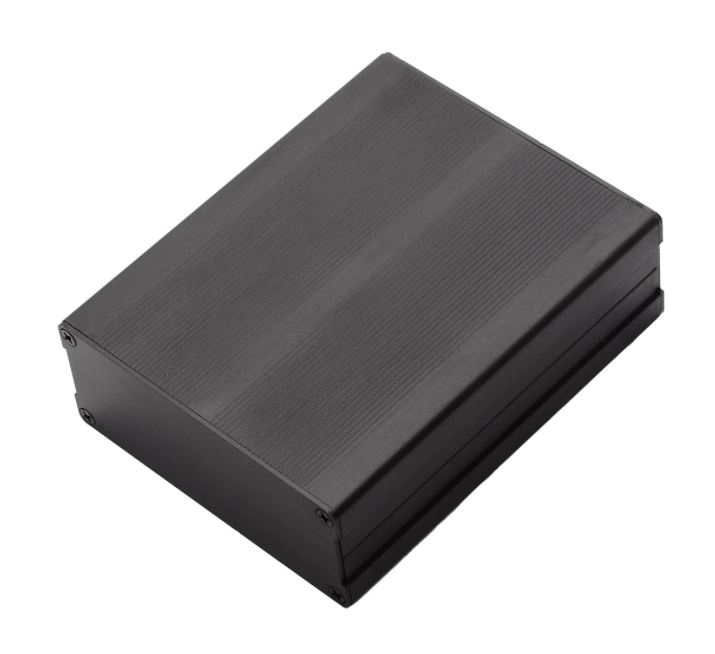
\includegraphics[scale=0.25]{model}
	\end{center}

	\columnbreak

	\section{Feature Overview}
	$\Delta$0:3 is packed with features such as:
	\begin{itemize}
		\item 5 to 120 second timer, with minimum of 0 seconds and a maximum of 24 hours.
		\item \textit{Atmega2560} microprocessor.
		\item Internal 20A max output \textit{18650} battery.
		\item 200W output.
		\item LCD display.
		\item Bluetooth remote controll.
		\item Constant voltage mode.
		\item Constant current mode.
		\item Resistance checking.
		\item In depth parameter monitoring.
		\item Audio cues.
	\end{itemize}
	A comprehensive list of features can be found below.
\end{multicols}

\section{Specs}
\begin{center}
	\textbf{Default Operating Conditions}\\
	\begin{tabular}{ |p{5cm}||p{1.5cm}|p{1.5cm}|p{1cm}|p{1cm}|p{2cm}|}
		\hline
		\textbf{Parameter}&\textbf{Symbol}&\textbf{Nominal}&\textbf{Min}&\textbf{Max}&\textbf{Unit}\\
		\hline\hline
		Activation timer						&	T$_1$	&	60	&	5	&	120	&	s	\\
		Pulse timer\footnotemark[1]				&	T$_p$	&	0	&	0	&	1	&	s	\\
		Output shutdown timer\footnotemark[1]	&	T$_s$	&	$-$	&	1	&	120	&	s	\\
		\hline
		Input voltage		&	V$_{in}$&12 or 3.6&	3	&	35	&	V	\\
		Output voltage		& 	V$_o$	&	$-$	&	$-$	&	40	&	V	\\
		Output current		&	I$_o$	&	$-$	&	$-$	&	5	&	A	\\
		Output power		&	P$_o$	&	$-$	&		&	200	&	W	\\
		\hline
		Buzzer frequency	&	F$_b$	&	880	&	$-$	&	$-$	&	Hz	\\
		Bluetooth range 	&	R$_{bt}$&	$-$	&	$-$	&	10	&	m	\\

		\hline
	\end{tabular}
	\newline\newline\newline
	\textbf{Absolute Maximum Operating Conditions}\\
	\begin{tabular}{ |p{5cm}||p{1.5cm}|p{1.5cm}|p{1cm}|p{1cm}|p{2cm}|}
		\hline
		\textbf{Parameter}&\textbf{Symbol}&\textbf{Nominal}&\textbf{Min}&\textbf{Max}&\textbf{Unit}\\
		\hline\hline
		Activation timer\footnotemark[2]	&	T$_1$	&	0	&	$-$	&	24	&	s, h	\\
		Pulse timer\footnotemark[1]\footnotemark[2]				&	T$_p$	&	0	&	0	&	1	&	s	\\
		Output shutdown timer\footnotemark[1]\footnotemark[2]	&	T$_s$	&	$-$	&	1	&	120	&	s	\\

		\hline
	\end{tabular}
\end{center}
\footnotetext[1]{Minimum is applicable only if the option is enabled.}
\footnotetext[2]{Some values denoted with \footnotemark[1] can be accessed by changing the settings or entering specific secret activation codes.}


\section{Firmware Features}
\begin{itemize}
	\item Bluetooth remote control.
	
	Set the \textit{Activation} switch to \textit{Armed} position for the unit to be activated remotely via bluetooth.
	\item Programmable output wattage.
	\item Programmable output voltage.
	\item Timed activation.
	\item Automatic fuse resistance check.
	\item Calibrator for output cable resistance.
	
	The user would have to manually enter the resistance of the output wires leading to and back from the fuse in order to have accurate power regulation.
	\item Password protected access, activation, and or deactivation.
	
	Passwords are stored on the Atmega EEPROM.
	\item Timed pulse setting for outputting current for a selected time.
	\item Timer post-countdown for measuring when the fuse blows out.
	\item Fuse current, voltage potential, resistance, and output power display.
	\item Stealth mode, shuts screen and any LEDs down during operation.
	\item Battery voltage display.



\end{itemize}



\section{Hardware Features}
\begin{itemize}
	\item \textit{Atmega2560} microprocessor.
	\item OLED or LCD display.
	
	Size debatable.
	\item Bluetooth module allowing for remote controll of the unit.
	\item External power connection.
	\item Internal \textit{18650} battery.
	
	Independant internal power allowing for a fully integrated operation of the unit. A switch allows you to select either internal or external 	battery mode.
	\item Boost converter to step up input voltage.
	\item PWM late stage MOSFET voltage regulator to step down output voltage and controll the output power.
	\item \textit{ACS712} or \textit{ACS758} hall effect current sensor for measuring output current.
	\item Internal battery charging protection.
	\item Buck converters for powering internal devices.
	\item Rotary encoder for navigating menus.
	\item External USB connector allowing for easy interface for reflashing firmware without disassembling the unit.
	\item Three pole DPDT
	\item Buzzer.
	\item Reverse polarity protection.
	\item GX16 connectors.
	\item Extruded aluminium case.
\end{itemize}

\section{Settings}
$\Delta$0-3 contains a number of useful settings in order to provide more controll of the unit to the user.

\begin{itemize}
	\item Bluetooth options.
	\item Speaker options.
\end{itemize}


\section{Considered Features}

\begin{itemize}
	\item SMT components

	Pros:
	\begin{itemize}
		\item Smaller form factor.
	\end{itemize}
	Cons:
	\begin{itemize}
		\item Requiring ordering of new parts and additional costs.
		\item Questionable ability to solder them.
	\end{itemize}
\end{itemize}

\section{Circuit Diagram}

\section{Internal Specifications}
\begin{center}
	\textbf{Internal Component Operating Conditions}\\
	\begin{tabular}{ |p{5cm}||p{1.5cm}|p{1.5cm}|p{1cm}|p{1cm}|p{2cm}|}
		\hline
		\textbf{Parameter}&\textbf{Symbol}&\textbf{Nominal}&\textbf{Min}&\textbf{Max}&\textbf{Unit}\\
		\hline\hline
		PWM frequency		& f$_{pwm}$	&	16	&	$-$	&	$-$	&	kHz	\\
		PWM duty cycle		& D$_{pwm}$	&	100	&	0	&	$-$	&	\%	\\
		\hline
	\end{tabular}
\end{center}



\section{Bill of Materials}
%To purchase:
Already acquired:

\begin{itemize}
	\item Extruded aluminium enclosure, 120x97x40.
	\item PCB.
	\item 1.8" LCD.
	\item 12 button keypad.
	\item DPDT switch, optional protextive cover.
	\item Buck converters.
	\item Boost converter/s.
	\item 18650 battery (x2).
	\item 18650 battery charging protection.
	\item 18650 battery holder.
	\item Bluetooth module.
	\item USB female connector.
	\item Hall current sensor.
	\item Voltage sensors (x2).
	\item MOSFETs.
	\item Rotary encoder.
	\item XH-25 pin headers.
	\item Atmega2560 arduino compatible board.
	\item Necessary caps and resistors.
	\item DPDT mini switches.
	\item Relays.
	\item LEDs.
	\item Buzzer.
\end{itemize}




\end{document}